\section{Exercise 3}

\subsection{Instruction}

If a carrier wave meets an ionospheric layer with a refractive index of 0, then
the group velocity tends to zero and the phase velocity tends to infinity as the
wave is reflected off the layer. What electron density $\eta_e$ would be required
for reflection at the GPS L1 frequency? Research typical electron density values
to determine whether there is any chance of such a reflection occurring. What
$\eta_e$ is required for reflection of the Ham Radio band at 50 MHz? What are the
chances of reflection at this frequency? For all reflections, assume a normally
incident wave (a wave with zenith angle 0).

\subsection{Solution}

The index of refraction can be, generally, written as

\begin{equation}
	\eta = \sqrt{1 - \frac{\eta_e e^2}{4 \pi^2 f^2 \epsilon_0 m}}
	= \sqrt{1 - \frac{40.3 \eta_e}{f^2}}
	\label{eq:refraction_index}
\end{equation}

where $\eta_e$ is the electron density, $e$ is the charge magnitude of electron,
$\epsilon_0$ is the permitibity of free space and $m$ is the mass of electron.
If the right hand side of \ref{eq:refraction_index} is close to 1, then it is
possible to use the following approximation.

\begin{equation}
	\eta = 1 - \frac{40.3 \eta_e}{f^2}
	\label{eq:refraction_index_approx}
\end{equation}

As it can be observed in Figure~\ref{fig:ex3_electron_density_iono}, the maximum
electron density one can get is in the neighborhood of $~10^{12} [m^{-3}]$. Thus,
the refraction index for a GPS signal can be modeled as \ref{eq:refraction_index_approx}
since $\eta \approx 1$ at those frequencies.

\begin{figure}[H]
	\centering
	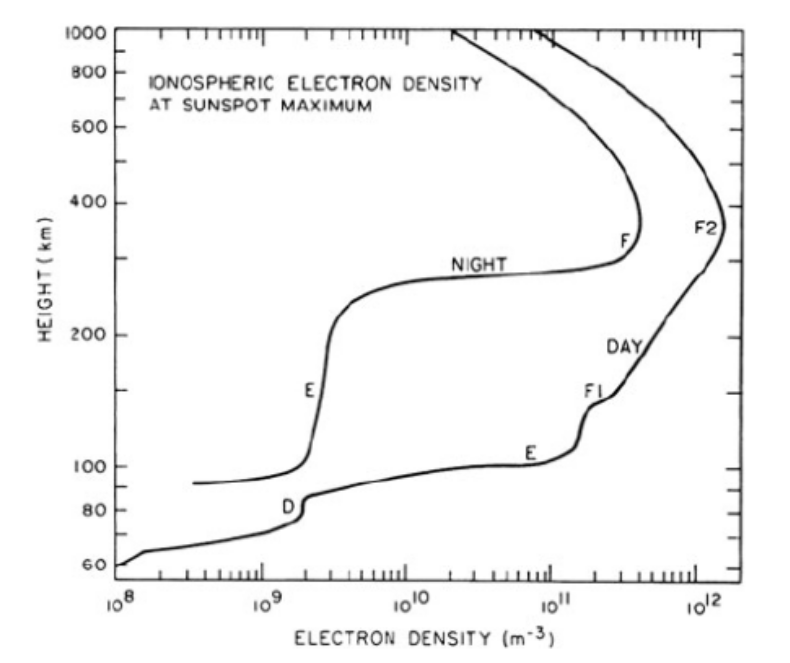
\includegraphics[width=0.9\textwidth]{figs/electron_density_iono.png}
	\caption{Idealized electron density distribution in the Earth’s ionosphere.
		The curves indicate thedensities to be expected at sunspot maximum in temperate
		latitudes. Peak sunspot activity occursat 11-year intervals, most recently
		peaking in 2001 (cycle 23) and 2012 (cycle 24). Cycle 24 wasabout a year late
		and rather weak [see Janardhan et al. (2015)]. From J. V. Evans and T. Hagfors,
		Radar Astronomy, 1968. McGraw-Hill Education}
	\label{fig:ex3_electron_density_iono}
\end{figure}

The electron density one would require for a signal at $f = 1575.42 MHz$ to be
reflected is close to $\eta_e = 6 \times 10^{16} [m^{-3}]$.

However, if the signal was at a frequency of $50MHz$, the electron density
necessary for it to be reflected is $\eta_e = 6 \times 10^{13} [m^{-3}]$.
Note that in this case, the electron density required for the signal to be
reflected is much closer to the maximum shown by the graph. Nevertheless,
the refraction index for the Ham Radio when the electron density is at its maximum
is $\eta \approx 0.98$. So, it is not likely for signals at this frequencies to
be reflected.

The calculations show that $f \approx 6 MHz$ is the critical frequency at which
the ionosphere starts fully reflecting the signals.
